\chapter{Wazuh}
\section{Entstehung}

\section{Aufbau}
Wazuh basiert auf dem \acrfull{elk} Stack. 
Es ist ein Plugin, welches in den \acrshort{elk} Stack integriert ist und mithilfe von Agents auf den Computern Logdateien sammelt.

\begin{figure}[H]
    \centering
    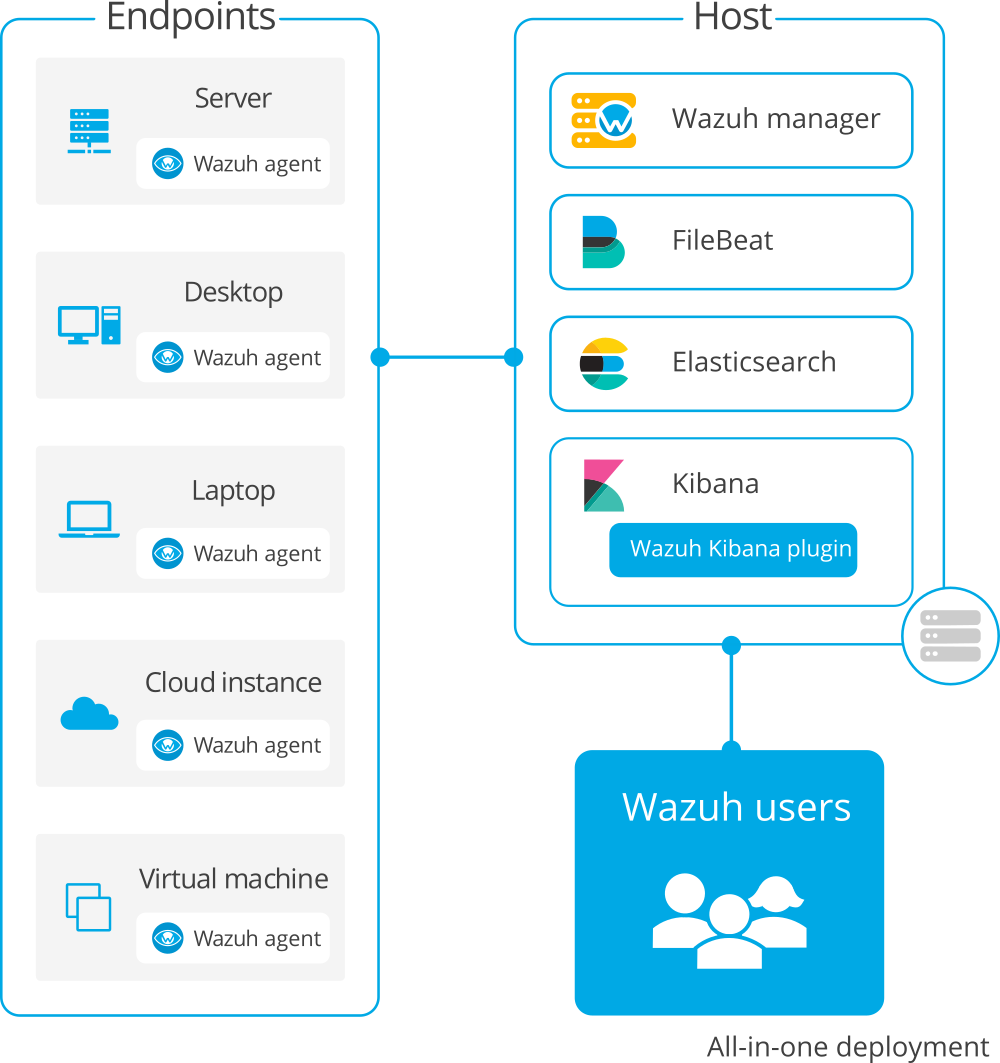
\includegraphics[width=0.7\linewidth]{../img/aufbau-wazuh.png}
    \caption{Übersicht Wazuh}
\end{figure}
%TODO: Cite

\subsection{Wazuh Manager}
Der Wazuh Manager wird auf einem Linux Server installiert.
Der Wazuh Manager beinhaltet den kompletten \acrshort{elk} Stack und das Wazuh Plugin. 

\subsection{Wazuh Agent}
